% begin module second-derivative-test
\begin{frame}
This gives us a new way of checking if critical points are local maxima or local minima:

\vspace{.3in}

The Second Derivative Test

Suppose $f''$ is exists near $c$.
\begin{enumerate}
\item  If $f'(c) = 0$ and $f''(c) > 0$, then $f$ has a local minimum at $c$.
\item  If $f'(c) = 0$ and $f''(c) < 0$, then $f$ has a local maximum at $c$.
\end{enumerate}
\uncover<2->{%
\begin{columns}[c]
\column{.3\textwidth}
\psset{xunit=1cm, yunit=1cm}
\begin{pspicture}(-0.5,-0.5)(3.4,2.7)
\tiny
\psaxes[ticks=none, labels=none]{<->}(0,0)(-0.5,-0.5)(3.3,2.6)
\fcLabels{3.3}{2.6}
%Function formula: -5/2-2 ((x) (x))+6 (x)
\psplot[linecolor=red, plotpoints=1000]{0.381966011}{2.618033989}{x 6 mul x x mul -2 mul add -2.5 add }
\psline[linestyle=dashed](1.5, 2)(1.5, 0)
\fcFullDot{1.5}{2}
\psline[linecolor=\fcColorTangent](-0.1,2)(2.9,2)
\tiny
\rput[t](1.5, -0.1){$c$}
\end{pspicture}

%\ 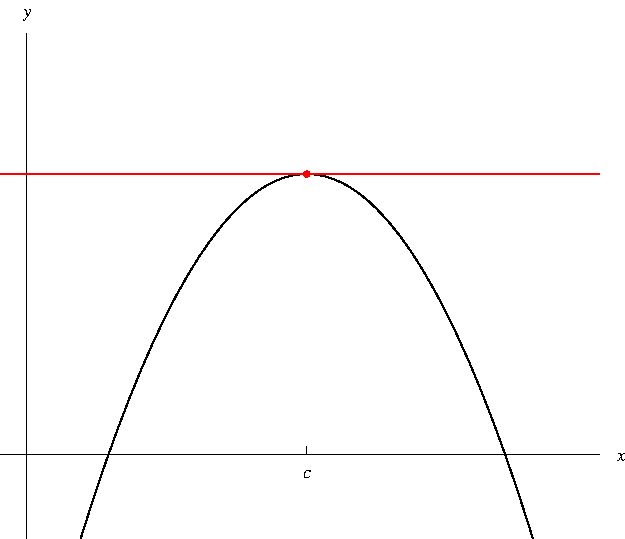
\includegraphics[height=3.5cm]{curve-sketching/pictures/04-03-secondderiv.pdf}%
\column{.7\textwidth}
\begin{itemize}
\item  $f'(c) = 0$, so $f$ has a horizontal tangent at $c$.
\item  $f''(c) < 0$, so $f$ is concave down near $c$.
\item  This means $f$ lies below its horizontal tangent.
\item  This means $f(c)$ is a local maximum.
\end{itemize}
\end{columns}
}%
\end{frame}
% end module second-derivative-test
